\section{Analisi}
\subsection{Casi d'uso}
I casi d'uso rappresentano uno strumento fondamentale nell'analisi dei requisiti di un sistema \textit{software}. Essi descrivono 
le interazioni tra gli utenti (o altri sistemi esterni) e il sistema in esame, illustrando come questo debba comportarsi per 
soddisfare le esigenze degli \textit{stakeholder}.\\
Ogni caso d'uso riporta:
\begin{itemize}
    \item \textbf{Attore}: attori coinvolti nel caso d'uso;
    \item \textbf{Descrizione}: descrizione del caso d'uso;
    \item \textbf{Pre-condizione}: condizioni vere prima del verificarsi del caso d'uso;
    \item \textbf{Post-condizione}: condizioni vere dopo il verificarsi del caso d'uso;
    \item \textbf{Scenario}: sequenza specifica di eventi che si verifica quando un attore interagisce con il sistema 
                             per raggiungere un obiettivo;
\end{itemize}
Gli attori che ho identificato sono:
\begin{itemize}
    \item \textbf{Utente non autenticato}: utente che non ha completato la procedura di \textit{login}, può essere un cliente o un agente;
    \item \textbf{Agente}: utente autenticato e riconosciuto dal sistema come agente aziendale;
    \item \textbf{Agente autenticato come cliente}: agente che ha selezionato un cliente e vuole operare all'interno dell'\textit{app} come il cliente selezionato.
\end{itemize}
Nelle sezioni seguenti, esamineremo in dettaglio i casi d'uso, che ho identificato durante lo studio del capitolato del progetto.

\subsubsection{UC 1 - \textit{Login}}
\begin{figure}[H]
    \vspace{2em}
    \centering
    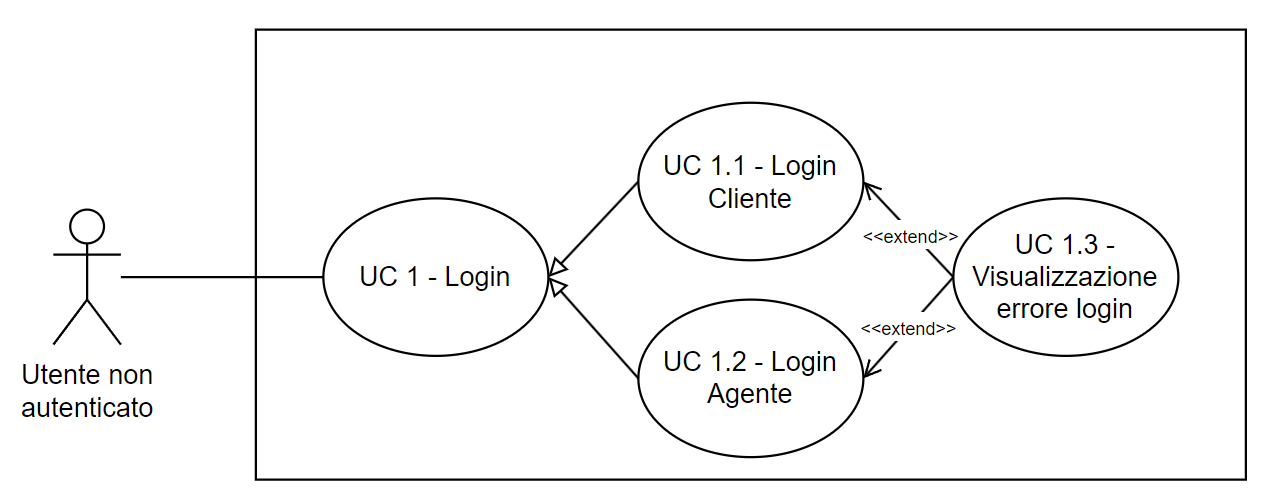
\includegraphics[width=0.75\columnwidth]{img/usecase/UC 1.png}
    \caption{\textit{Use Case} 1: \textit{Login} Utente}
    \label{fig:uc_1}
\end{figure}

\begin{usecase}{ 1}{\textit{Login} utente}
    \usecaseactors{Utente non autenticato.}
    \usecasedesc{L'utente ha inserito \textit{username} e \textit{password} per autenticarsi nell'\textit{app}.}
    \usecasepre{L'utente ha avviato l'\textit{app}.}
    \usecasepost{L'utente è autenticato nel sistema o ha ricevuto un errore.}
    \usecasescen{
        \begin{itemize}
            \item L'utente visualizza la schermata di \textit{login} di {\movi};
            \item L'utente inserisce lo \textit{username};
            \item L'utente inserisce la \textit{password};
            \item L'utente preme il pulsante per effettuare il \textit{login};
            \item L'utente viene autenticato ed entra nell'applicazione.
        \end{itemize}}
    \label{uc:uc_1}
\end{usecase}

\begin{usecase}{ 1.1}{\textit{Login} cliente}
    \usecaseactors{Utente non autenticato.}
    \usecasedesc{L'utente è un cliente dell'azienda e vuole autenticarsi nell'\textit{app}.}
    \usecasepre{L'utente ha avviato l'\textit{app}.}
    \usecasepost{L'utente è autenticato come cliente nel sistema o ha ricevuto un errore. Viene portato 
                 nella \textit{\texttt{Homepage}} e nulla cambia rispetto la vecchia versione dell'\textit{app}.}
    \usecasescen{
        \begin{itemize}
            \item L'utente visualizza la schermata di \textit{login} di {\movi};
            \item L'utente inserisce lo \textit{username};
            \item L'utente inserisce la \textit{password};
            \item L'utente preme il pulsante per effettuare il \textit{login};
            \item L'utente viene autenticato e visualizza la \textit{\texttt{Homepage}} dell'applicazione.
        \end{itemize}}
    \label{uc:uc_1.1}
\end{usecase}

\begin{usecase}{ 1.2}{\textit{Login} agente}
    \usecaseactors{Utente non autenticato.}
    \usecasedesc{L'utente è un agente dell'azienda e vuole autenticarsi nell'\textit{app}.}
    \usecasepre{L'utente ha avviato l'\textit{app}.}
    \usecasepost{L'utente è autenticato come agente nel sistema o ha ricevuto un errore. Viene portato 
                 nella \texttt{\textit{Homepage} Agenti}.}
    \usecasescen{
        \begin{itemize}
            \item L'utente visualizza la schermata di \textit{login} di {\movi};
            \item L'utente inserisce lo \textit{username};
            \item L'utente inserisce la \textit{password};
            \item L'utente preme il pulsante per effettuare il \textit{login};
            \item L'utente viene autenticato e visualizza la \texttt{\textit{Homepage} Agenti} dell'applicazione.
        \end{itemize}}
    \label{uc:uc_1.2}
\end{usecase}

\begin{usecase}{ 1.3}{Visualizzazione errore \textit{login}}
    \usecaseactors{Utente non autenticato.}
    \usecasedesc{L'utente vuole autenticarsi nell'\textit{app} ma ha inserito \textit{username} o \textit{password} non validi.}
    \usecasepre{L'utente ha avviato l'operazione di \textit{login}.}
    \usecasepost{L'utente visualizza un messaggio che lo avvisa del fallimento dell'operazione di \textit{login}.}
    \usecasescen{
        \begin{itemize}
            \item L'utente visualizza la schermata di \textit{login} di {\movi};
            \item L'utente inserisce lo \textit{username};
            \item L'utente inserisce la \textit{password};
            \item L'utente preme il pulsante per effettuare il \textit{login};
            \item L'utente visualizza un errore.
        \end{itemize}}
    \label{uc:uc_1.3}
\end{usecase}
\subsubsection{UC 2 - Operazioni disponibili nella \texttt{Homepage Agenti}}
\begin{figure}[H]
    \vspace{2em}
    \centering
    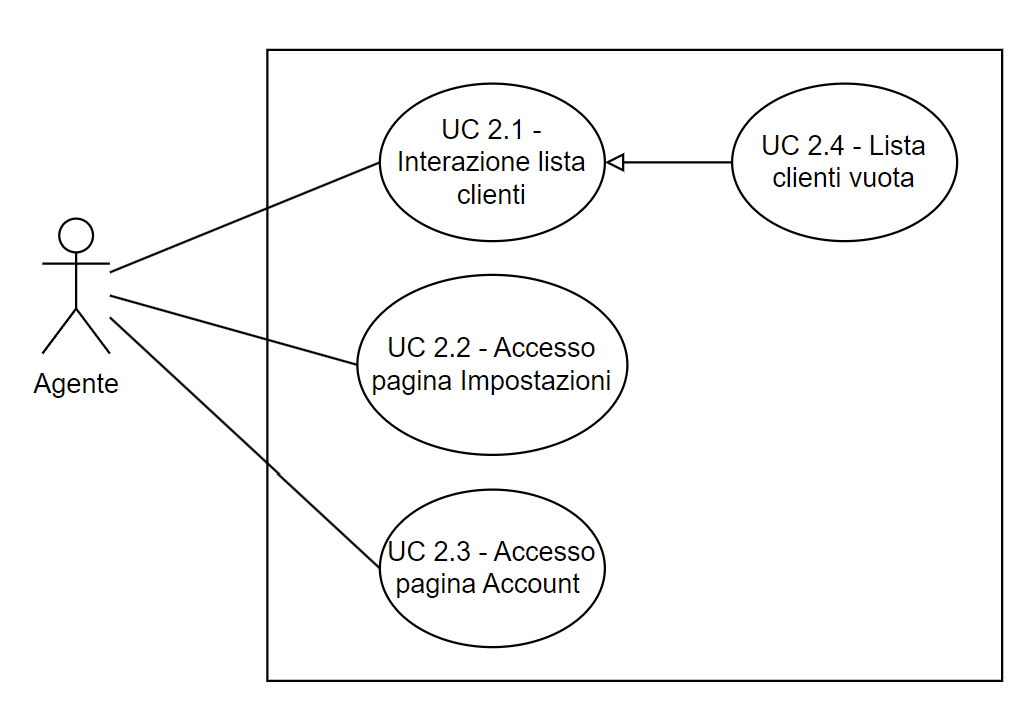
\includegraphics[width=0.75\columnwidth]{img/usecase/UC 2.png}
    \caption{\textit{Use Case} 2: Operazioni disponibili nella \texttt{Homepage Agenti}}
    \label{fig:uc_2}
\end{figure}

\begin{usecase}{ 2.2}{Accesso pagina \texttt{Impostazioni}}
    \usecaseactors{Agente.}
    \usecasedesc{L'agente, cliccando nell'apposito menu il pulsante "Impostazioni", viene spostato nella pagina \texttt{Impostazioni}.}
    \usecasepre{L'utente si è autenticato con successo ed e stato riconosciuto come agente, quindi visualizza la 
                \texttt{Homepage Agenti}.}
    \usecasepost{L'agenti viene spostato nella nella pagina \texttt{Impostazioni}.}
    \usecasescen{
        \begin{itemize}
            \item L'agente visualizza la \texttt{Homepage Agenti};
            \item L'agente visualizza il menu;
            \item L'agente clicca il pulsante "Impostazioni";
            \item L'agente viene spostato nella pagina \texttt{Impostazioni}.
        \end{itemize}}
    \label{uc:uc_2.2}
\end{usecase}

\begin{usecase}{ 2.3}{Accesso pagina \texttt{Account}}
    \usecaseactors{Agente.}
    \usecasedesc{L'agente, cliccando nell'apposito menu il pulsante "\textit{Account}", viene spostato nella pagina \texttt{Account}.}
    \usecasepre{L'utente si è autenticato con successo ed e stato riconosciuto come agente, quindi visualizza la 
                \texttt{Homepage Agenti}.}
    \usecasepost{L'agenti viene spostato nella nella pagina \texttt{Account}.}
    \usecasescen{
        \begin{itemize}
            \item L'agente visualizza la \texttt{Homepage Agenti};
            \item L'agente visualizza il menu;
            \item L'agente clicca il pulsante "\textit{Account}";
            \item L'agente si sposta nella pagina \texttt{Account}.
        \end{itemize}}
    \label{uc:uc_2.3}
\end{usecase}

\begin{usecase}{ 2.4}{Lista clienti vuota}
    \usecaseactors{Agente.}
    \usecasedesc{L'agente che ha una lista clienti vuota visualizza il messaggio 
                 "nessun cliente trovato".}
    \usecasepre{
        \begin{itemize}
            \item L'utente si è autenticato con successo ed e stato riconosciuto come agente, quindi visualizza la 
                \texttt{Homepage Agenti}
            \item La lista clienti è vuota.
        \end{itemize}}
    \usecasepost{L'agente visualizza il messaggio "nessun cliente trovato".}
    \usecasescen{
        \begin{itemize}
            \item L'agente visualizza la \texttt{Homepage Agenti}
            \item La lista clienti è vuota;
            \item L'agente visualizza il messaggio "nessun cliente trovato" al posto della lista.
        \end{itemize}}
    \label{uc:uc_2.4}
\end{usecase}
\subsubsection{UC 2.1 - Interazioni con la lista clienti}
\begin{figure}[H]
    \vspace{2em}
    \centering
    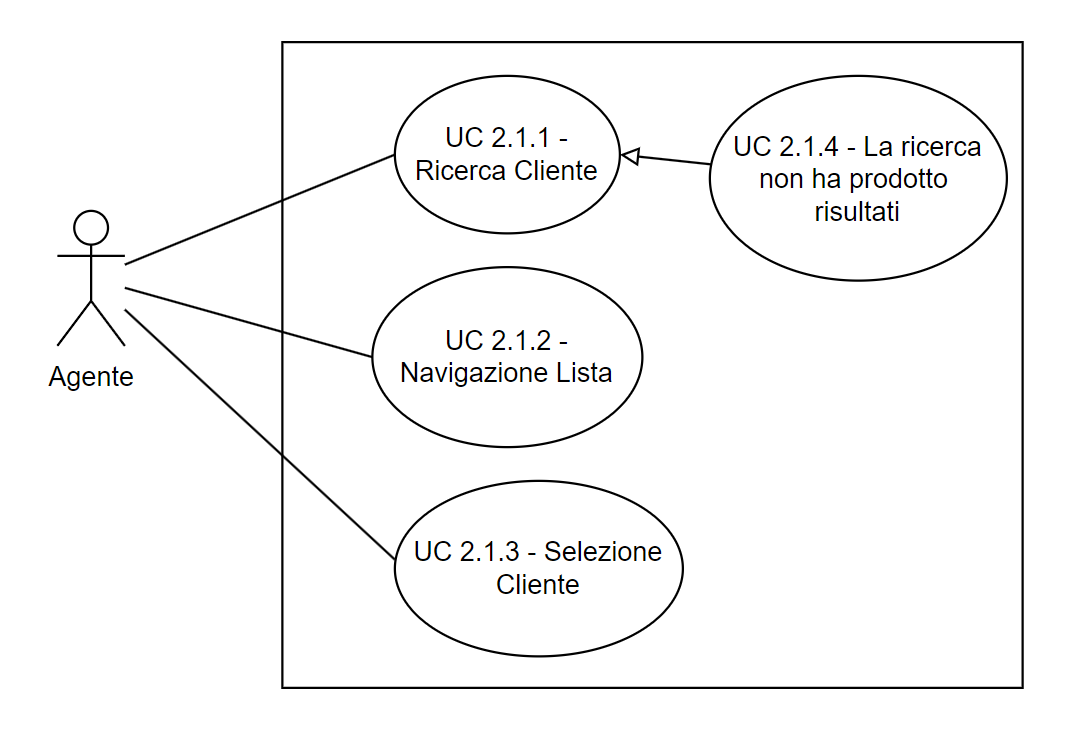
\includegraphics[width=0.75\columnwidth]{img/usecase/UC 2.1.png}
    \caption{\textit{Use Case} 2.1: Interazioni con la lista clienti}
    \label{fig:uc_2.1}
\end{figure}

\begin{usecase}{ 2.1.1}{Ricerca cliente}
    \usecaseactors{Agente.}
    \usecasedesc{L'agente ricerca un cliente specifico all'interno della lista clienti.}
    \usecasepre{
        \begin{itemize}
            \item L'utente si è autenticato con successo ed è stato riconosciuto come agente, quindi visualizza la 
                \texttt{\textit{Homepage} Agenti};
            \item La lista clienti non è vuota.
    \end{itemize}}
    \usecasepost{L'agente visualizza il cliente ricercato.}
    \usecasescen{
        \begin{itemize}
            \item L'agente visualizza la \texttt{\textit{Homepage} Agenti};
            \item L'agente visualizza la lista clienti;
            \item L'agente ricerca un cliente nella lista clienti;
            \item L'agente visualizza il cliente ricercato.
        \end{itemize}}
    \label{uc:uc_2.1.1}
\end{usecase}

\begin{usecase}{ 2.1.2}{Navigazione lista}
    \usecaseactors{Agente.}
    \usecasedesc{L'agente naviga la lista che contiene tutti i clienti dell'agente.}
    \usecasepre{
        \begin{itemize}
            \item L'utente si è autenticato con successo ed è stato riconosciuto come agente, quindi visualizza la 
                \texttt{\textit{Homepage} Agenti};
            \item La lista clienti non è vuota.
    \end{itemize}}
    \usecasepost{L'agente è riuscito a navigare nella lista.}
    \usecasescen{
        \begin{itemize}
            \item L'agente visualizza la \texttt{\textit{Homepage} Agenti};
            \item L'agente naviga la lista visualizzando i clienti contenuti.
        \end{itemize}}
    \label{uc:uc_2.1.2}
\end{usecase}

\begin{usecase}{ 2.1.3}{Selezione cliente}
    \usecaseactors{Agente.}
    \usecasedesc{L'agente seleziona un cliente per operare nell'\textit{app} come il cliente selezionato.}
    \usecasepre{
        \begin{itemize}
            \item L'utente si è autenticato con successo ed è stato riconosciuto come agente, quindi visualizza la 
                \texttt{\textit{Homepage} Agenti};
            \item La lista clienti non è vuota.
    \end{itemize}}
    \usecasepost{L'agente viene spostato nella \textit{\texttt{Homepage}} e può operare nell'\textit{app} come il cliente selezionato.}
    \usecasescen{
        \begin{itemize}
            \item L'agente visualizza la \texttt{\textit{Homepage} Agenti};
            \item L'agente visualizza la lista clienti;
            \item L'agente seleziona un cliente;
            \item L'agente viene spostato nella \textit{\texttt{Homepage}};
            \item L'agente può operare nell'\textit{app} come il cliente selezionato.
        \end{itemize}}
    \label{uc:uc_2.1.3}
\end{usecase}

\begin{usecase}{ 2.1.4}{La ricerca non ha prodotto risultati}
    \usecaseactors{Agente.}
    \usecasedesc{La ricerca di un cliente specifico all'interno della lista clienti non ha prodotto risultati.}
    \usecasepre{
        \begin{itemize}
            \item L'utente si è autenticato con successo ed è stato riconosciuto come agente, quindi visualizza la 
                \texttt{\textit{Homepage} Agenti};
            \item La lista clienti non è vuota;
            \item L'agente ricerca un cliente.
    \end{itemize}}
    \usecasepost{L'agente visualizza il messaggio "nessun cliente trovato".}
    \usecasescen{
        \begin{itemize}
            \item L'agente visualizza la \texttt{\textit{Homepage} Agenti};
            \item L'agente visualizza la lista clienti;
            \item L'agente ricerca un cliente nella lista clienti;
            \item La ricerca non produce risultati;
            \item L'agente visualizza il messaggio "nessun cliente trovato".
        \end{itemize}}
    \label{uc:uc_2.1.4}
\end{usecase}
\subsubsection{UC 3 - Operazioni disponibili nella \texttt{\textit{Homepage} Agenti} 
               autenticati come clienti}
\begin{figure}[H]
    \vspace{2em}
    \centering
    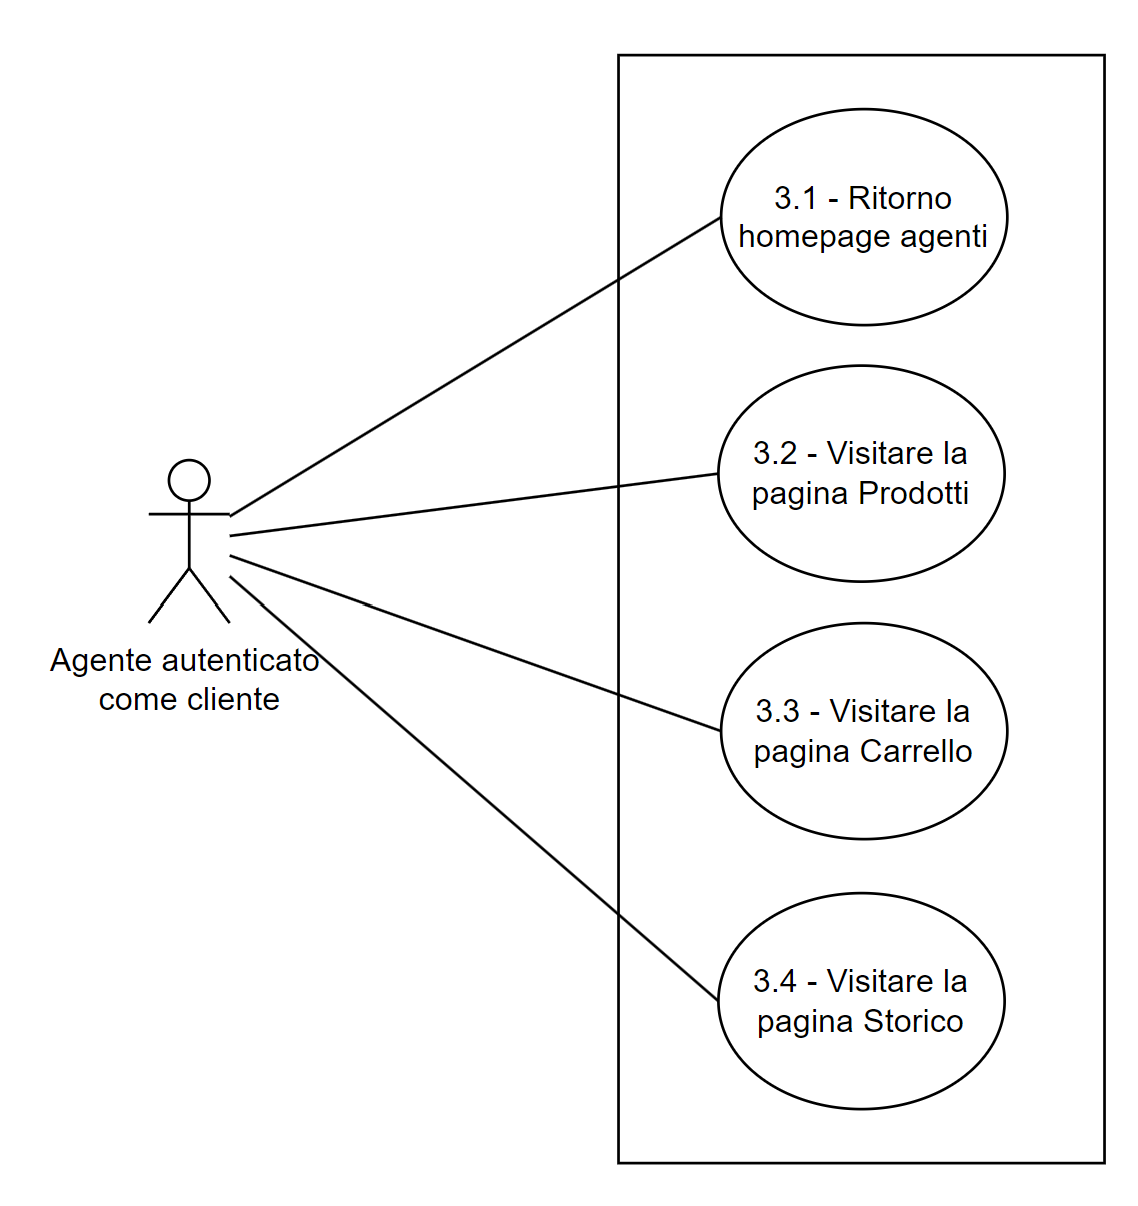
\includegraphics[width=0.75\columnwidth]{img/usecase/UC 3.png}
    \caption{\textit{Use Case} 3: Operazioni disponibili nella \texttt{\texttt{\textit{Homepage} Agenti}}}
    \label{fig:uc_3}
\end{figure}

\begin{usecase}{ 3.1}{Ritorno \texttt{\textit{Homepage} Agenti}}
    \usecaseactors{Agente.}
    \usecasedesc{L'agente, cliccando nell'apposito menu il pulsante "\textit{Homepage} Agenti", ritorna alla 
                 \texttt{\textit{Homepage} Agenti}.}
    \usecasepre{L'agente ha selezionato un cliente dalla lista.}
    \usecasepost{L'agente si è spostato nella \texttt{\textit{Homepage} Agenti}.}
    \usecasescen{
        \begin{itemize}
            \item L'agente seleziona un cliente della lista;
            \item L'agente viene spostato nella \textit{\texttt{Homepage}};
            \item L'agente può operare nell'\textit{app} come il cliente selezionato;
            \item L'agente preme il pulsante "\textit{Homepage} Agenti";
            \item L'agente ritorna alla \texttt{\textit{Homepage} Agenti}.
        \end{itemize}}
    \label{uc:uc_3.1}
\end{usecase}

\begin{usecase}{ 3.2}{Visitare la pagina \texttt{Prodotti}}
    \usecaseactors{Agente.}
    \usecasedesc{L'agente, cliccando nell'apposito menu il pulsante "Prodotti", può operare nella pagina 
                 \texttt{Prodotti} come il cliente selezionato.}
    \usecasepre{L'agente ha selezionato un cliente dalla lista.}
    \usecasepost{L'agente si è spostato nella pagina \texttt{Prodotti}.}
    \usecasescen{
        \begin{itemize}
            \item L'agente seleziona un cliente della lista;
            \item L'agente viene spostato nella \textit{\texttt{Homepage}};
            \item L'agente preme il pulsante "Prodotti";
            \item L'agente viene spostato nella pagina \texttt{Prodotti} dove può operare come il cliente selezionato.
        \end{itemize}}
    \label{uc:uc_3.2}
\end{usecase}

\begin{usecase}{ 3.3}{Visitare la pagina \texttt{Carrello}}
    \usecaseactors{Agente.}
    \usecasedesc{L'agente, cliccando nell'apposito menu il pulsante "Carrello", può operare nella pagina 
                 \texttt{Carrello} come il cliente selezionato.}
    \usecasepre{L'agente ha selezionato un cliente dalla lista.}
    \usecasepost{L'agente si è spostato nella pagina \texttt{Carrello}.}
    \usecasescen{
        \begin{itemize}
            \item L'agente seleziona un cliente della lista;
            \item L'agente viene spostato nella \textit{\texttt{Homepage}};
            \item L'agente preme il pulsante "Carrello";
            \item L'agente viene spostato nella pagina \texttt{Carrello} dove può operare come il cliente selezionato.
        \end{itemize}}
    \label{uc:uc_3.3}
\end{usecase}

\begin{usecase}{ 3.4}{Visitare la pagina \texttt{Storico}}
    \usecaseactors{Agente.}
    \usecasedesc{L'agente, cliccando nell'apposito menu il pulsante "Storico", può operare nella pagina 
                 \texttt{Storico} come il cliente selezionato.}
    \usecasepre{L'agente ha selezionato un cliente dalla lista.}
    \usecasepost{L'agente si è spostato nella pagina \texttt{Storico}.}
    \usecasescen{
        \begin{itemize}
            \item L'agente seleziona un cliente della lista;
            \item L'agente viene spostato nella \textit{\texttt{Homepage}};
            \item L'agente preme il pulsante "Storico";
            \item L'agente viene spostato nella pagina \texttt{Storico} dove può operare come il cliente selezionato.
        \end{itemize}}
    \label{uc:uc_3.4}
\end{usecase}
\subsubsection{UC 4 - Cambio tema}
\begin{figure}[H]
    \vspace{2em}
    \centering
    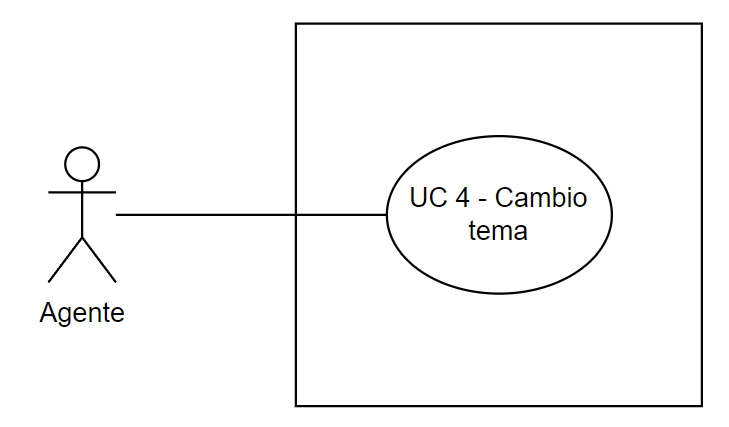
\includegraphics[width=0.75\columnwidth]{img/usecase/UC 4.png}
    \caption{\textit{Use Case} 4: Cambio tema}
    \label{fig:uc_4}
\end{figure}

\begin{usecase}{ 4}{Cambio tema}
    \usecaseactors{Agente.}
    \usecasedesc{L'agente cambia il tema dell'applicazione in chiaro o scuro.}
    \usecasepre{L'agente, dalla \texttt{\textit{Homepage} Agenti}, cliccando nell'apposito menu il pulsante "Impostazioni", si 
                sposta nella pagina \texttt{Impostazioni}.}
    \usecasepost{L'agente ha cambiato il tema dell'\textit{app}.}
    \usecasescen{
        \begin{itemize}
            \item L'agente si trova nella \texttt{\textit{Homepage} Agenti};
            \item L'agente preme il pulsante "Impostazioni" dal menu;
            \item L'agente viene spostato nella pagina \texttt{Impostazioni};
            \item L'agente cambia il tema dell'applicazione.
        \end{itemize}}
    \label{uc:uc_4}
\end{usecase}
\subsubsection{UC 5 - \textit{Logout}}
\begin{figure}[H]
    \vspace{2em}
    \centering
    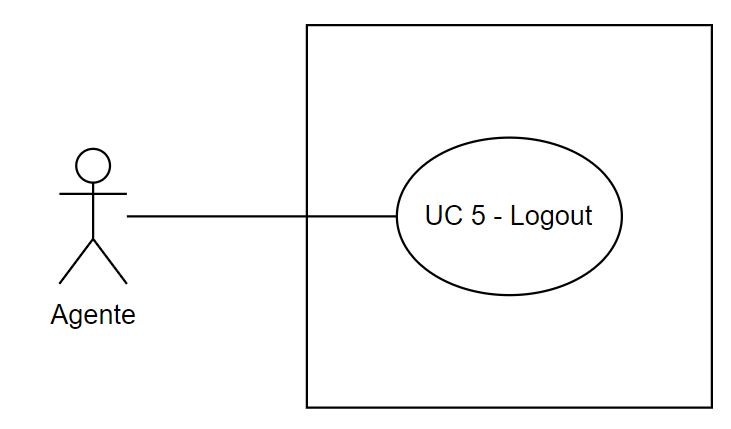
\includegraphics[width=0.75\columnwidth]{img/usecase/UC 5.png}
    \caption{\textit{Use Case} 5: \textit{Logout}}
    \label{fig:uc_5}
\end{figure}

\begin{usecase}{ 5}{\textit{Logout}}
    \usecaseactors{Agente.}
    \usecasedesc{L'agente effettua la procedura di \textit{logout}.}
    \usecasepre{L'agente, dalla \texttt{Homepage Agenti}, cliccando nell'apposito menu il pulsante "\textit{Account}", si 
                sposta nella pagina \texttt{Account}.}
    \usecasepost{L'agente ha effettuato il \textit{logout} e torna un utente non autenticato. 
                 L'agente viene spostato alla pagina di \textit{login}.}
    \usecasescen{
        \begin{itemize}
            \item L'agente si trova nella \texttt{Homepage Agenti};
            \item L'agente preme il pulsante "\textit{Account}" dal menu;
            \item L'agente viene spostato nella pagina \texttt{Account};
            \item L'agente effettua il \textit{logout};
            \item L'agente torna un utente non autenticato;
            \item L'agente viene spostato alla pagina di \textit{login}
        \end{itemize}}
    \label{uc:uc_5}
\end{usecase}

\subsection{Requisiti funzionali e non funzionali}
L'analisi dei casi d'uso rappresenta un punto di partenza fondamentale per l'identificazione e la definizione dei requisiti 
funzionali e non funzionali del progetto.\\
I requisiti funzionali descrivono le funzionalità specifiche che il sistema deve offrire, dettagliando il comportamento atteso 
in risposta alle diverse interazioni degli utenti. 
I requisiti non funzionali, d'altra parte, definiscono le caratteristiche qualitative del sistema, come prestazioni, 
sicurezza, usabilità e scalabilità. Sebbene non sempre esplicitamente evidenti nei casi d'uso, questi requisiti 
sono spesso impliciti nelle aspettative degli utenti e nelle condizioni operative del sistema.
Ho assegnato ad ogni requisito un codice identificativo, che riporta:
\begin{itemize}
    \item \textbf{F, V, Q, U}: F rappresenta i requisiti funzionali, V i requisiti non funzionali di vincolo, Q i 
          requisiti non funzionali qualitativi e U i 
          requisiti non funzionali di usabilità;
    \item \textbf{O, D}: O per i requisiti obbligatori, D per quelli desiderabili;
    \item \textbf{id}: numero identificativo del requisito;
\end{itemize}
Per ogni requisito viene fornita anche una descrizione e la fonte da cui è tratto.
Le fonti che vengono riportate nella tabella indicano da dove ho ricavato il requisito descritto, principalmente 
troviamo:
\begin{itemize}
    \item \textbf{UC}: i casi d'uso precedentemente descritti hanno portato alla definizione del requisito descritto;
    \item \textbf{Capitolato}: il requisito descritto è stato ricavato dal capitolato del progetto;
    \item \textbf{\textit{Tutor}}: il requisito descritto è stato ricavato da colloqui avuti con il \textit{tutor} aziendale 
          durante il tirocinio;
    \item \textbf{\textit{Studente}}: il requisito descritto è stato ricavato da personali considerazioni sul progetto.
\end{itemize}

\begin{center}
    \rowcolors{1}{}{tableGray}
    \begin{longtable}{|p{2.25cm}|p{7.75cm}|p{2.25cm}|}
    \hline
    %\rowcolor{hyperColor!5}
    \multicolumn{1}{|c|}{\textbf{Requisito}} & \multicolumn{1}{c|}{\textbf{Descrizione}} & \multicolumn{1}{c|}{\textbf{Fonte}}\\
    \hline 
    \endfirsthead
    \rowcolor{white}
    \multicolumn{3}{c}{{\bfseries \tablename\ \thetable{} -- Continuo della tabella}}\\
    \hline
    %\rowcolor{hyperColor!5}
    \multicolumn{1}{|c|}{\textbf{Requisito}} & \multicolumn{1}{c|}{\textbf{Descrizione}} & \multicolumn{1}{c|}{\textbf{Fonte}}\\
    \hline 
    \endhead
    \hline
    \rowcolor{white}
    \multicolumn{3}{|r|}{{Continua nella prossima pagina...}}\\
    \hline
    \endfoot
    \endlastfoot
    
    FO1 & Un utente deve poter effettuare il \textit{login} ed essere automaticamente riconosciuto come cliente & UC 1.1, Capitolato \\
    FO1.1 & Un cliente deve essere spostato nella \texttt{Homepage} in seguito al \textit{login} & UC 1.1, Capitolato \\
    FO1.2 & Un cliente non deve poter notare nessuna differenza rispetto alla precedente versione dell'\textit{app} & Capitolato \\
    FO2 & Un utente deve poter effettuare il \textit{login} ed essere automaticamente riconosciuto come agente & UC 1.2, Capitolato \\
    FO2.1 & Un agente deve essere spostato nella \texttt{Homepage Agenti} in seguito al \textit{login} & UC 1.2, Studente \\
    FO3 & Un utente deve visualizzare un messaggio d'errore se le credenziali sono errate & UC 1.3, Studente \\
    FO4 & Un agente deve poter visualizzare una lista con i suoi clienti & Capitolato \\
    FD4.1 & Un agente deve poter ricercare un cliente all'interno della lista dei suoi clienti & UC 2.1.1, \textit{Tutor} \\
    FO4.2 & Un agente deve poter navigare la lista dei suoi clienti & UC 2.1.2, Capitolato \\
    FO4.3 & Un agente deve poter selezionare dalla lista uno dei suoi clienti & UC 2.1.3, Capitolato \\
    FO4.4 & Un agente deve visualizzare un messaggio d'errore che riporta la frase "nessun cliente trovato" se la lista clienti è vuota & UC 2.4, \textit{Tutor} \\
    FD4.5 & Un agente deve visualizzare un messaggio d'errore che riporta la frase "nessun cliente trovato" se la ricerca clienti non ha prodotto risultati & UC 2.1.4, \textit{Tutor} \\
    FO4.6 & Un agente deve essere spostato nella pagina \texttt{Homepage} dopo aver selezionato un cliente dalla lista & UC 2.1.3, Studente \\
    FO4.7 & Un agente deve essere autenticato come il cliente selezionato dopo aver selezionato un cliente dalla lista & UC 2.1.3, Capitolato \\
    FD5 & Un agente deve poter visualizzare un menu nella \texttt{Homepage Agenti} & Studente \\
    FD5.1 & Un agente deve poter premere il pulsante "Impostazioni" dal menu nella \texttt{Homepage Agenti} & UC 2.2, Studente \\
    FD5.2 & Un agente deve essere spostato nella pagina \texttt{Impostazioni} dopo aver premuto il pulsante "Impostazioni" & UC 2.2, Studente \\
    FD5.3 & Un agente deve poter premere il pulsante "\textit{Account}" dal menu nella \texttt{Homepage Agenti} & UC 2.3, Studente \\
    FD5.4 & Un agente deve essere spostato nella pagina \texttt{Account} dopo aver premuto il pulsante "\textit{Account}" & UC 2.3, Studente \\
    FO6 & Un agente autenticato come cliente deve poter visualizzare un menu nella \texttt{Homepage} & Studente \\
    FD6.1 & Un agente autenticato come cliente deve poter ritornare alla \texttt{Homepage Agenti} premendo 
            il pulsante "\textit{Homepage} Agenti" nel menu della \texttt{Homepage} & 3.1, Studente \\
    FD6.2 & Un agente autenticato come cliente deve essere spostato nella pagina \texttt{Prodotti} premendo 
            il pulsante "Prodotti" nel menu della \texttt{Homepage} & 3.2, Capitolato \\
    FD6.2.1 & Un agente autenticato come cliente deve poter operare come il cliente selezionato nella pagina \texttt{Prodotti} & 3.2, Capitolato \\
    FD6.3 & Un agente autenticato come cliente deve essere spostato nella pagina \texttt{Carrello} premendo 
            il pulsante "Carrello" nel menu della \texttt{Homepage} & 3.3, Capitolato \\
    FD6.3.1 & Un agente autenticato come cliente deve poter operare come il cliente selezionato nella pagina \texttt{Carrello} & 3.3, Capitolato \\
    FD6.4 & Un agente autenticato come cliente deve essere spostato nella pagina \texttt{Storico} premendo 
            il pulsante "Storico" nel menu della \texttt{Homepage} & 3.4, Capitolato \\
    FD6.4.1 & Un agente autenticato come cliente deve poter operare come il cliente selezionato nella pagina \texttt{Storico} & 3.4, Capitolato \\
    FD7.1 & Un agente deve poter modificare il tema impostando il tema chiaro dalla pagina \texttt{Impostazioni} & UC 4, \textit{Tutor} \\
    FD7.2 & Un agente deve poter modificare il tema impostando il tema scuro dalla pagina \texttt{Impostazioni} & UC 4, \textit{Tutor} \\
    FO7.3 & Un agente non deve poter modificare la propria schermata d'avvio dalla pagina \texttt{Impostazioni} & Studente \\
    FD8 & Un agente deve poter effettuare il \textit{logout} dalla pagina \texttt{Account} & UC 5, \textit{Tutor} \\
    QO1 & Insieme al modulo deve essere consegnato anche un manuale tecnico & Capitolato, \textit{Tutor} \\
    QO2 & Insieme al modulo deve essere consegnato anche un manuale utente & Capitolato, \textit{Tutor} \\
    UO1 & Un agente deve visualizzare il suo nome all'interno della schermata \texttt{Homepage Agenti} & Capitolato, Studente \\
    UO2 & Un agente deve visualizzare il nome del cliente selezionato all'interno della schermata \texttt{Homepage} & Capitolato, Studente \\
    UO3 & Ogni voce della lista deve riportare alcune informazioni del cliente & \textit{Tutor} \\
    UO3.1 & Ogni voce della lista deve riportare il nome del cliente & \textit{Tutor} \\
    UO3.2 & Ogni voce della lista deve riportare l'indirizzo del cliente & \textit{Tutor} \\
    UD4 & L'applicazione deve essere disponibile nella lingua italiana & \textit{Tutor} \\
    UD5 & L'applicazione deve essere disponibile nella lingua inglese & \textit{Tutor} \\
    UD6 & Deve essere possibile ricercare un cliente nelle lista attraverso l'uso di una \textit{search bar} & \textit{Tutor} \\
    UD7 & Durante la digitazione del parametro di ricerca i risultati devono essere filtrati anche per i parametri parziali & \textit{Tutor} \\
    UD8 & Durante la ricerca i clienti devono essere filtrati secondo il parametro digitato dall'agente & \textit{Tutor} \\
    UD9 & Lo stile dell'applicazione deve essere compatibile con dispositivi \textit{tablet} & Capitolato, \textit{Tutor} \\
    VO1 & Il modulo deve utilizzare i \textit{database} di {\movi} apportando eventuali modifiche alla struttura & Capitolato, \textit{Tutor} \\
    VO2 & Il modulo deve estendere le \gls{api} esistenti sviluppate in .NET & Capitolato, \textit{Tutor} \\
    VO3 & Il modulo deve estendere le interfacce esistenti sviluppate in React Native & Capitolato, \textit{Tutor} \\
    \hline
    \hiderowcolors
    \caption{Tabella del tracciamento dei requisiti funzionali e non funzionali.}
    \label{tab:requisiti_funzionali}
    \end{longtable}
\end{center}

Ho qui riportato una tabella che riepiloga i requisiti precedentemente descritti.

\begin{center}
    \rowcolors{1}{}{tableGray}
    \begin{longtable}{|>{\centering\arraybackslash}p{2.25cm}|>{\centering\arraybackslash}p{4.75cm}|>{\centering\arraybackslash}p{4.75cm}|>{\centering\arraybackslash}p{2.25cm}|}    \hline
    \multicolumn{1}{|c|}{\textbf{Tipologia}} & \multicolumn{1}{c|}{\textbf{Obbligatorio}} & \multicolumn{1}{c|}{\textbf{Desiderabile}} & \multicolumn{1}{c|}{\textbf{Totale}}\\ 
    \hline 
    \endfirsthead
    \rowcolor{white}
    \multicolumn{4}{c}{{\bfseries \tablename\ \thetable{} -- Continuo della tabella}}\\
    \hline
    \multicolumn{1}{|c|}{\textbf{Tipologia}} & \multicolumn{1}{c|}{\textbf{Obbligatorio}} & \multicolumn{1}{c|}{\textbf{Desiderabile}} & \multicolumn{1}{c|}{\textbf{Totale}}\\ \hline 
    \endhead
    \hline
    \rowcolor{white}
    \multicolumn{4}{|r|}{{Continua nella prossima pagina...}}\\
    \hline
    \endfoot
    \endlastfoot 

    % Insert your table rows here
    \textbf{Funzionale} & 13 & 17 & 30 \\
    \textbf{Di vincolo} & 3 & 0 & 3 \\
    \textbf{Qualitativi} & 2 & 0 & 2 \\
    \textbf{Usabilità} & 5 & 6 & 11 \\
    \textbf{Totale} & 23 & 23 & 46 \\

    \hline
    \hiderowcolors
    \caption{Riepilogo requisti}
    \label{tab:requisiti riassunto}
    \end{longtable}
\end{center}





